\documentclass[11pt]{scrartcl}
\usepackage[a4paper]{geometry}

\usepackage{graphicx}
%\graphicspath{ {./images/} }

\usepackage{fancyhdr}
\pagestyle{fancy}
\fancyhf{}
\fancyhead[L]{ECHOGRAPHIE} %Kopfzeile links
\fancyfoot[C]{\thepage}

\usepackage[utf8]{inputenc}
\usepackage{csquotes}
\usepackage[german]{babel}

\usepackage{setspace}

\usepackage{caption}
\usepackage{float}

\usepackage{hyperref}
\usepackage{pdfpages}

\hypersetup{
    pdftitle = {Echographie},
    pdfsubject = {Biomedizinischesystemtechnik Praktikum},
    pdfauthor = {Leona Köck, Chris Rüttimann},
    pdfkeywords = {} ,
    pdfcreator = {pdflatex},
    pdfproducer = {LaTeX with hyperref}
}

\usepackage[
    style=apa,
    backend=biber,
    sortcites=false,
    sorting=none,
    hyperref=true,
    backref=false
]{biblatex}
\usepackage{amsmath}
\usepackage[T1]{fontenc}
\addbibresource{test.bib}
\setlength{\parindent}{0in}


\begin{document}
    \pagenumbering{Alph}
% ---------------------
% Titlepage
% ---------------------
    \begin{titlepage}
        \begin{center}
        {\LARGE OST Ostschweizer Fachhochschule}
            \\[1.5cm]
            \linespread{1.2}\large { Biomedizinischesystemtechnik Praktikum }

            \huge{\bfseries Echographie}
            \\%[1.5cm]
            \large{durchgeführt am 22. März 2021}
            \\[1.5cm]
   %         \linespread{1}
           
\includegraphics[width=8cm]{../images/ost_logo.eps}
           \\[1cm]
            {\small{Autoren}}\\
            {\Large{Leona Köck}}\\
            {\Large{Chris Rüttimann}}
            \\[1cm]

            \vspace*{\fill}
            \large{\today}
        \end{center}

    \end{titlepage}

% ---------------------
% Abstract
% ---------------------
    \pagenumbering{Roman}
 %   \pdfbookmark[section]{Abstract}{abstract}
 %   \section*{Abstract}
    \addtocounter{section}{0}

 %   \pagebreak
    \setstretch{1.25}
% ---------------------
% Table of contents
% ---------------------
    \tableofcontents
    \pagebreak


% ---------------------
% Body
% ---------------------
    \pagenumbering{arabic}

%    \section{Problem- und Zielvorstellung}
   
%    \section{Problemlösung}

    \section{Vorbereitung}
   
    Der Versuch wurde nach der Anleitung von \cite{Echographie} durchgeführt.
    Dafür wurden folgende Materialien benötigt:

    \begin{itemize}
        \item PC mit Software (Echo Wave II)
        \item Ultraschallgerät LogicScan der Firma Telemed
        \item Linear Array-Transducer mit 64 Elementen, 5-10MHz
        \item Ultraschall-Phantom
        \item Ultraschall-Gel
        
    \end{itemize}

    Zur Vorbereitung wurde mithilfe des Dokuments \cite{medUS} die folgenden Fragen beantwortet: %todo

    \begin{itemize}
        \item[a] Wie viel Zeit wird benötigt, um ein Echogramm aufzunehmen, das aus 64 einzelnen parallelen Linien besteht und eine Eindringtiefe von 75 mm aufweist?
        \item[] $c=1500m/s, n=64, l=0.075m$
        \item[] $t=\frac{l}{c}*n*2=\frac{0.075m*s}{1500m}*64*2=0.0064s$
        \item[b] Wie gross muss das Schallfenster beim linearen Array-Transducer sein, damit der ganze Array benützt werden kann (am Transducer nachmessen)?
                 Ist dieser Transducertyp günstig, um das Herz abzubilden?
        \item[]  Der Linearschallkopf arbeitet mit einer parallelen Schallausbreitung, dadurch entsteht ein rechteckiges Bild.
        Das Schallfenster entspricht also der Länge des Transducers selbst.
        Er benötigt dadurch eine recht grosse Fläche zu Ankoppelung, das ist ein Nachteil wenn nur begrenzter Platz zur Verfügung steht.
        Eine Untersuchung in knöchern geschützen Regionen wie
        beispielsweise das Herz ist daher nur sehr eingeschränkt möglich.
    \end{itemize}

    \section{Messungen und Ergebnisse}

    \subsection{Aufgabe D: Messungen am Phantom}
    Zuerst wurde das Gerät und die Software \emph{Echo Wave II} in Betrieb genommen.
    Das Ultraschallphantom ist eine Nachbildung, welche sich bei Ultraschallgeräten ähnlich verhält, wi der menschliche Körper.
    Meist wird es zur Kalibrierung vom Messgeräten eingesetzt, da der Abstand der Drähte im Innern exakt bekannt ist.

    \subsubsection{5 und 8 MHz, Dynamischer Fokus}

    Bei dieser Aufgabe wurden unterschiedliche Einstellungen bezüglich der Sendefrequenz als auch des Sendefokus des Transducers am Phantom getestet.
    Zuerst wurde mit dem linearen Array bei 5 MHz und einem Sendefokus von 15mm gemessen (Abbildung \ref{fig:D_5_15}).
    Der kleine weisse Pfeil an der linken Achse steht für den Sendefokus.
    Man erkennt, dass die Drähte in einer Tiefe von ca. 10mm sind.
    Da der Sendefokus tiefer liegt, werden sie nicht exakt abgebildet.
    Trotzdem stimmt die Abstandsmessung zwischen ihnen.

    Wird der Sendefokus auf 46mm erhöht (\autoref{fig:D_5_46}), erhält man wie erwartet ein schärferes Bild der
    Drähte in 46mm Tiefe.
    Die Drähte in 10mm Tiefe werden dann aber unscharf abgebildet.

    %done Bild 8MHz 46mm isch au 15mm Fokus, lömmer da eifach weg?
    % passt
    Bei erhöhter Sendefrequenz wird das Bild mit weniger Rauschen dargestellt (\autoref{fig:D_8_15}).

    \subsubsection{Ohne dynamische Fokussierung}

    Schaltet man den dynamischen Fokus aus (\autoref{fig:o_d_F}), sehen die Drähte teilweise mehr aus wie
    Dreiecke.
    Beim dynamischen Fokussieren wird der Effekt ausgenützt, welcher bei der sogenannten Schallbündelschwenkung zustande
    kommt.
    Mithilfe der Gruppenstrahlertechnik können die einzelnen Strahlen zeitverzögert oder phasengesteuert (geschwenkt)
    angesteuert werden.
    Dadurch entsteht ein Interferenzfeld im Prüfobjekt.
    Durch integrierte Software können dadurch Laufzeitdifferenzen berechnet und kompensiert werden.
    Weiter Informationen darüber sind unter \cite{gruppenstrahler} und \cite{arraytechnik} zu finden.

    %done: Erklärung dynamischer Fokus https://www.ndt.net/article/v05n09/waldron/waldron.htm#3

    \subsection{Aufabe E: Carotis und Farbdoppler-Aufnahme}

    Die Messung der Carotis Communis wurde mit dem linearen Array, sowie einer Sendefrequenz von 8MHz und
    Fokaldistanz von 15mm durchgeführt.
    Diese Untersuchung wird genutzt, um die Halsschlagader auf Gefässwandablagerungen, Verkalkungen und Störungen im
    Blutfluss zu untersuchen.
    Diese Werte können Hinweise auf ein Schlaganfall- oder Herzinfarktrisiko liefern.\\\\

    Die Halsschlagader abzubilden war für die Autoren nicht ganz einfach.
    Nach mehreren Versuchen und mit ausreichend Gel konnte dann dieses Bild erstellt werden:
    \autoref{images/E2_e}.
    Mit der Tiefenskala am linken Rand lässt sich ein Durchmesser von ca. 6.5mm der Carotis abschätzen.
    Aus den Ultraschall-Bildern geht hervor, dass es an dieser Stelle weder Erweitungen noch Verengungen
    oder Ablagerungen gibt.

    %done: meh Blabla?
    %todo, irgendwie hon mir nur farbdoppler aufnahmen aber koane ohne.... söllan ma dia zämafasssa?
    %\subsection{Aufgabe F: Farbdoppler-Aufnahme}


    \pagebreak

    \section*{Eigenständigkeitserklärung}
    \addcontentsline{toc}{section}{Eigenständigkeitserklärung}

    Hiermit bestätigen wir, dass wir diesen Bericht selbstständig und ohne fremde Hilfe verfasst haben.
    Alle verwendeten Quellen wurden entsprechend dem APA-Standard gekennzeichnet.
    \\[3cm]


    \begin{figure}[H]
        
\includegraphics[width=4cm]{.././images/Unterschrift_Leona.png}
    \end{figure}
    \begin{tabular}{@{} l@{}}
        \hline \\
        \makebox[6cm]{Leona Köck}\\[2cm]
    \end{tabular}


    \begin{figure}[H]
        
\includegraphics[width=4cm]{.././images/Unterschrift_Chris.png}
    \end{figure}
    \begin{tabular}{@{} l@{}}
        \hline\\
        \makebox[6cm]{Chris Rüttimann}
    \end{tabular}

    \pagebreak
% ---------------------
% References
% ---------------------
    %\printbibliography
    \addcontentsline{toc}{section}{Literaturverzeichnis}

% ---------------------
% List of figures
% ---------------------
    \listoffigures
    \addcontentsline{toc}{section}{Abbildungsverzeichnis}
    \pagebreak

% ---------------------
% List of tables
% ---------------------
%\listoftables



% ---------------------
% Anhang
% ---------------------
\appendix

    \section{Bilder Aufgabe D}

    \begin{figure}[H]
        \centering
        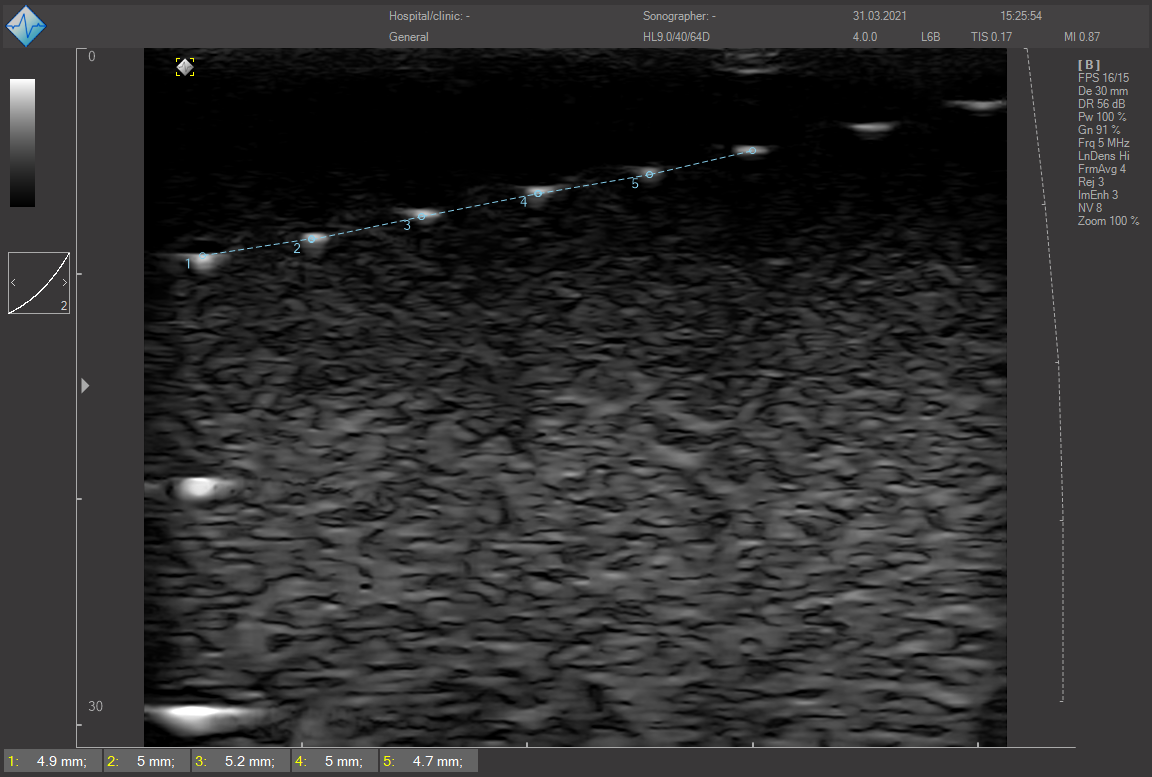
\includegraphics[height=8cm]{images/D_5_15_e}
        \caption{5MHz 15mm}
        \label{fig:D_5_15}
    \end{figure}

    \begin{figure}[H]
        \centering
        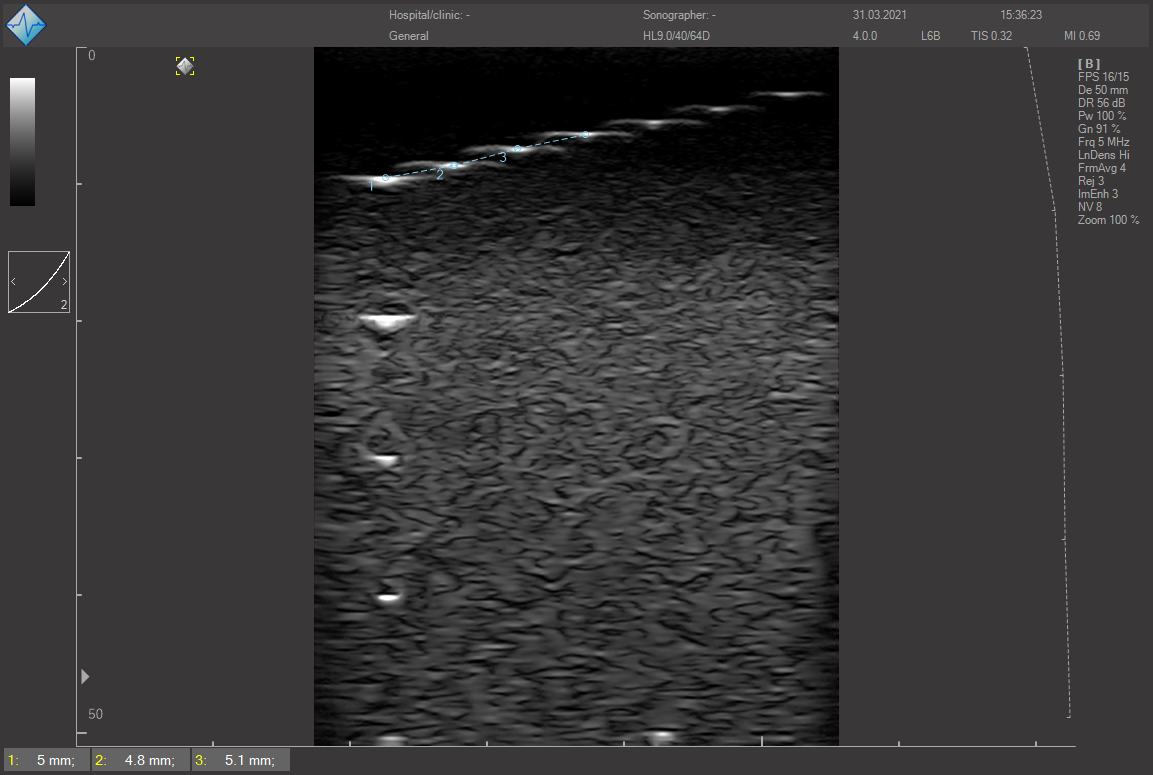
\includegraphics[height=8cm]{images/D_5_46_e}
        \caption{5MHz 46mm}
        \label{fig:D_5_46}
    \end{figure}

    \begin{figure}[H]
        \centering
        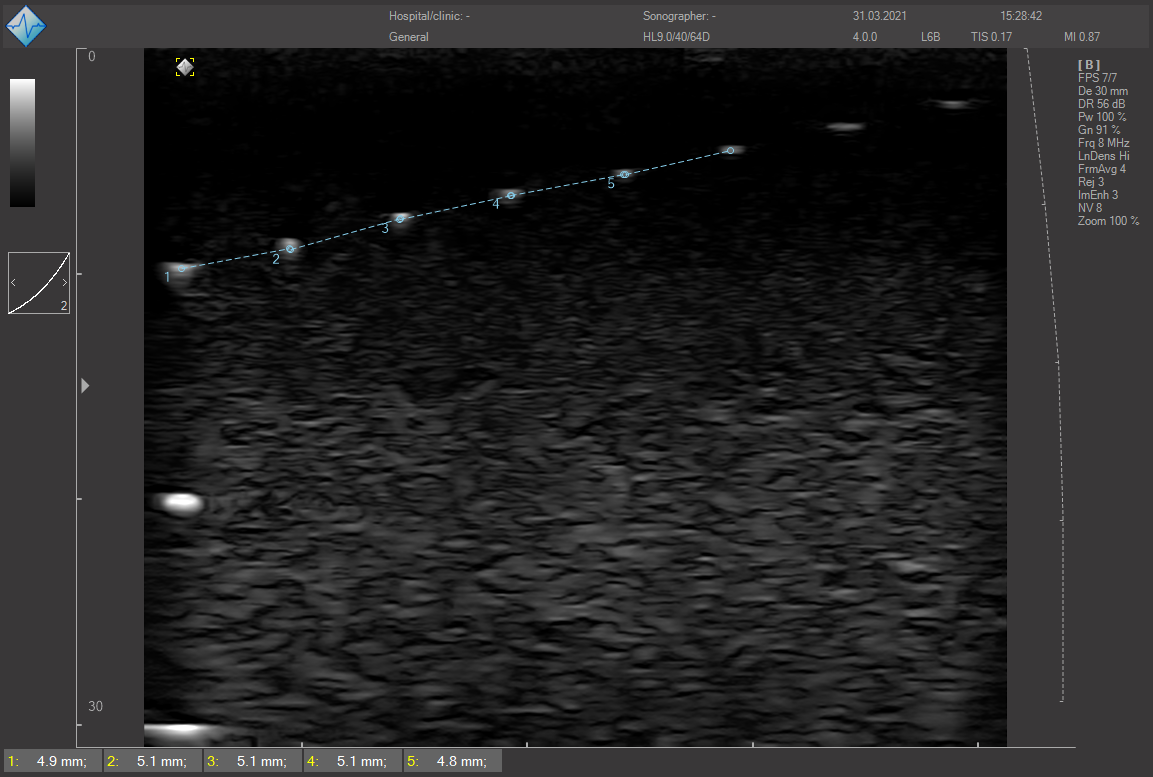
\includegraphics[height=8cm]{images/D_8_15_e}
        \caption{8MHz 15mm}
        \label{fig:D_8_15}
    \end{figure}

    \begin{figure}[H]
        \centering
        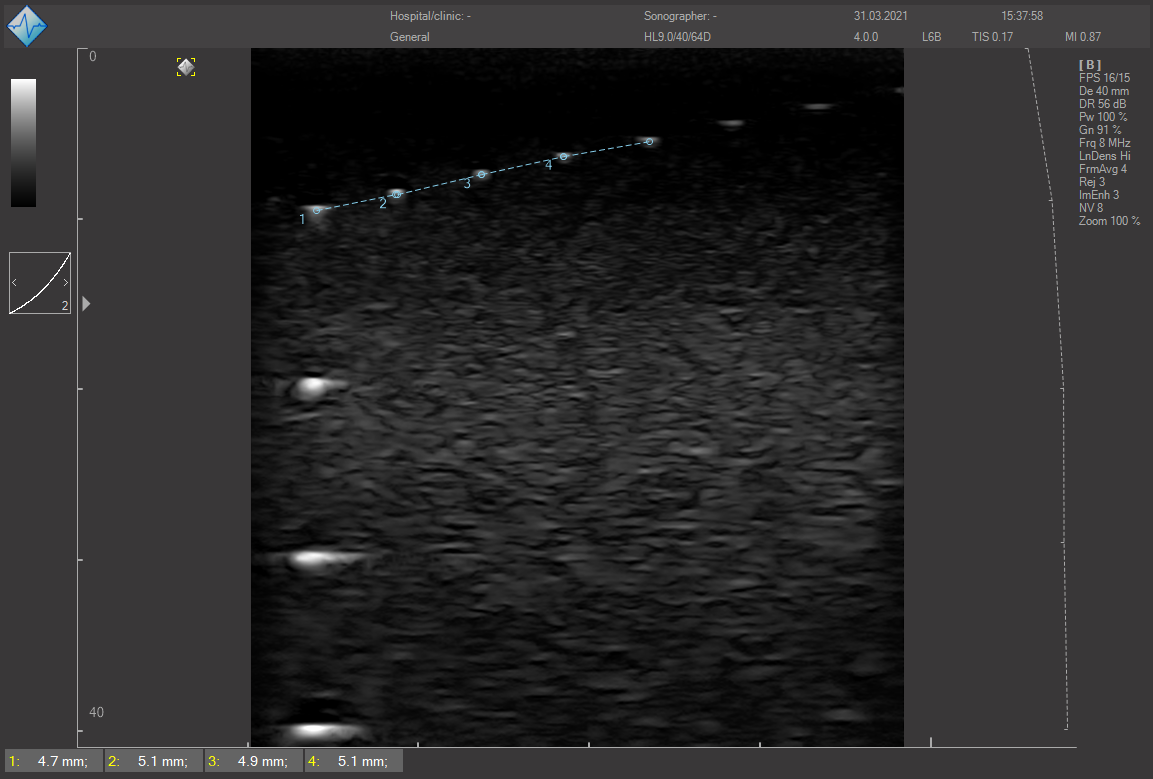
\includegraphics[height=8cm]{images/D_8_46_e}
        \caption{8MHz 46mm}
        \label{fig:D_8_46}
    \end{figure}

    \begin{figure}[H]
        \centering
        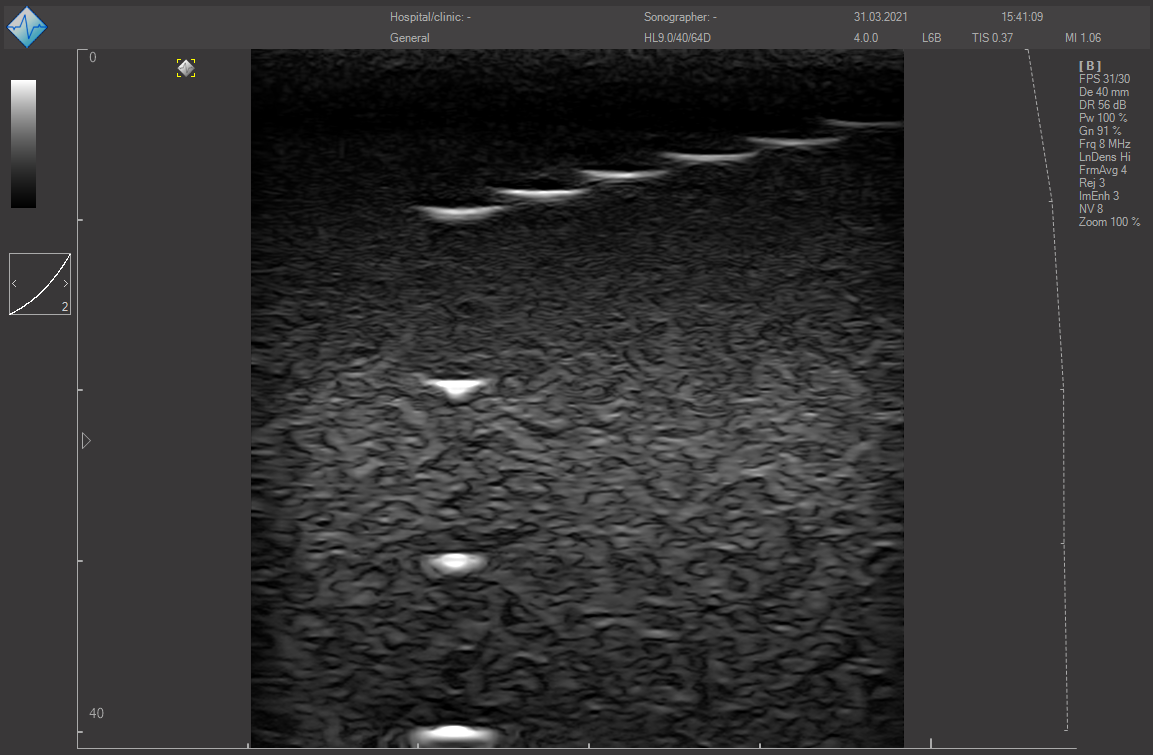
\includegraphics[height=8cm]{images/D_ohne_dynamisch_fokusiert_e}
        \caption{Ohne dynamischen Fokus}
        \label{fig:o_d_F}
    \end{figure}

    \begin{figure}[H]
        \centering
        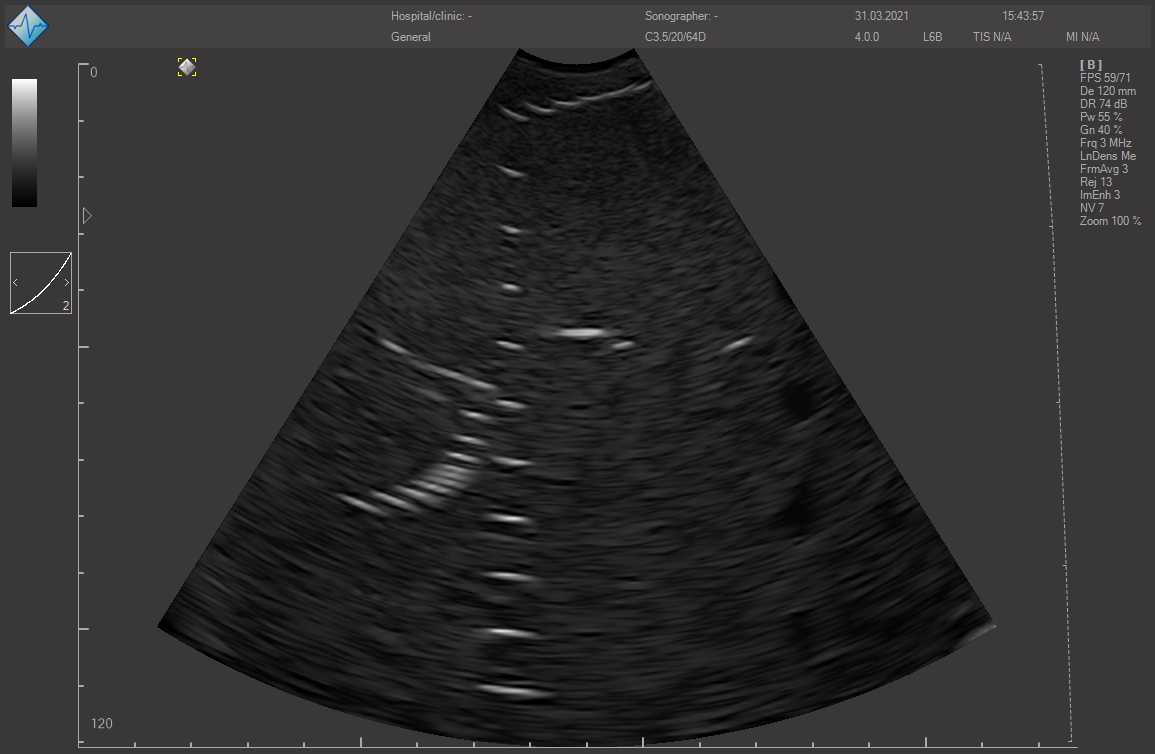
\includegraphics[height=8cm]{images/D_3_e}
        \caption{Curved Array}
        \label{fig:curvedArray}
    \end{figure}

    \section{Bilder Aufgabe E}

    \begin{figure}[H]
        \centering
        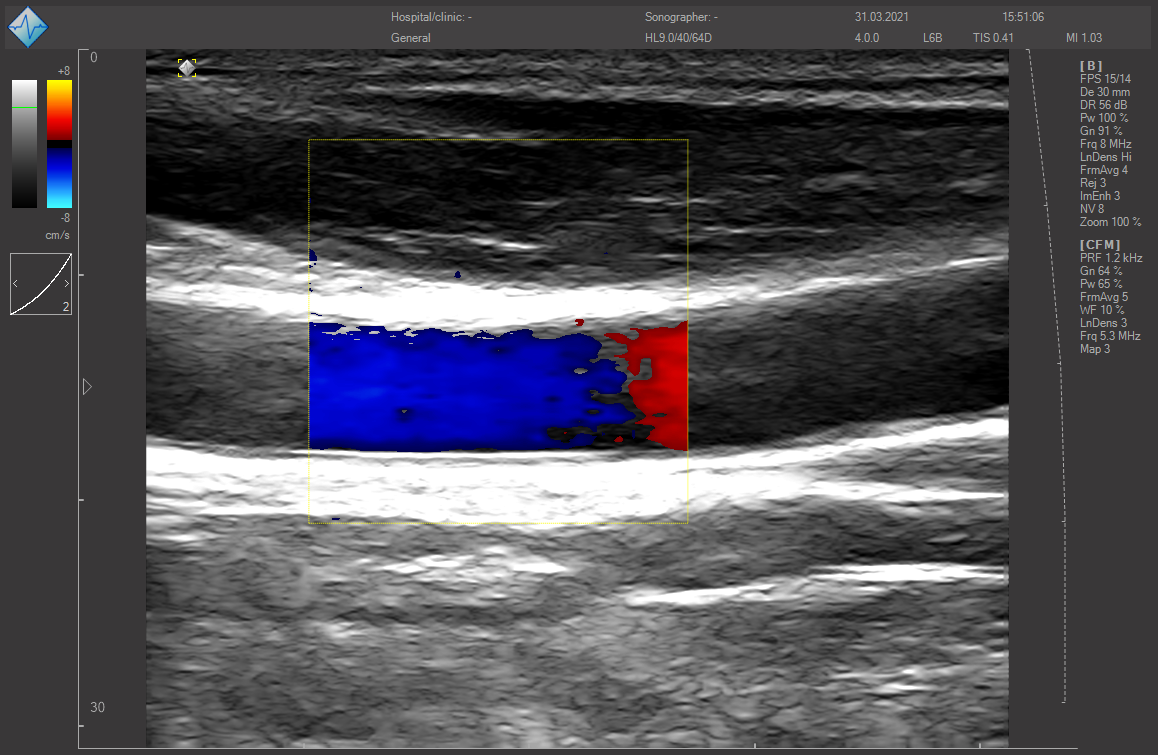
\includegraphics[height=8cm]{images/E1_e}
        \caption{Carotis 1}
        \label{fig:carotis1}
    \end{figure}

    \begin{figure}[H]
        \centering
        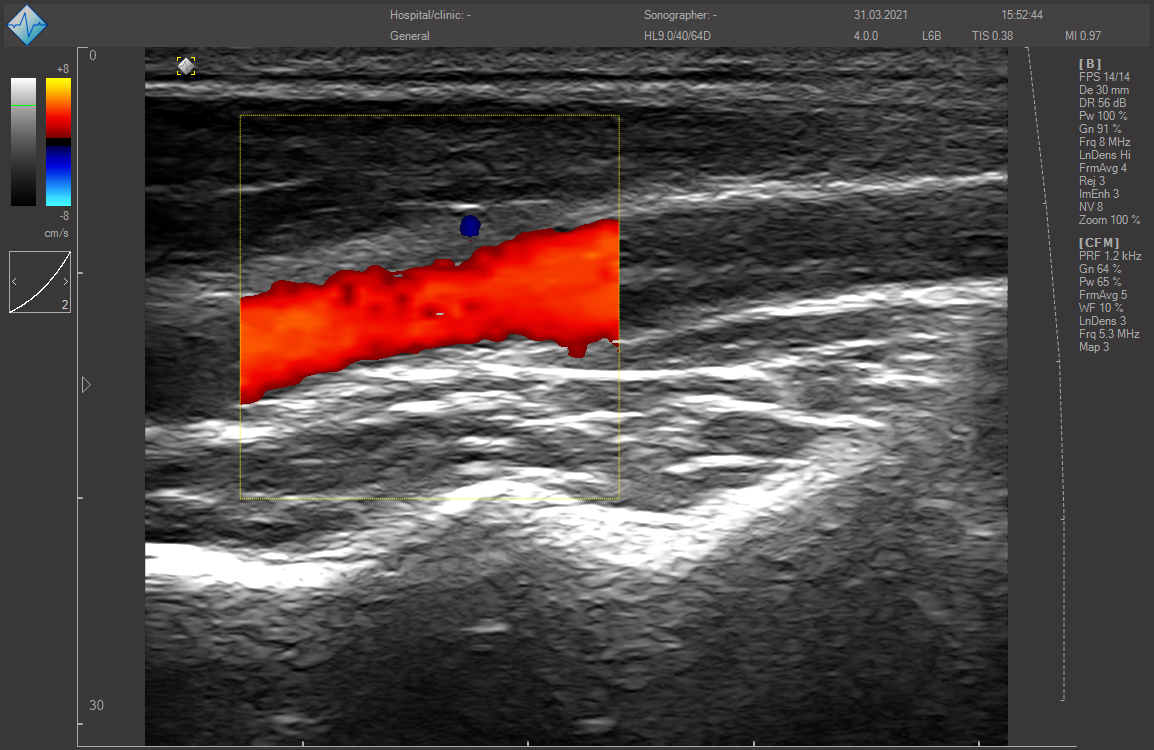
\includegraphics[height=8cm]{images/E2_e}
        \caption{Carotis 2}
        \label{fig:carotis2}
    \end{figure}

\end{document}